\documentclass[10pt]{article}
\advance\hoffset by -0.7 truein\relax


\usepackage{graphicx}
%\input{epsf}

\topmargin=-0.4in
%\leftmargin=-1in 
\textwidth=6.3in
\textheight=8.8in


\usepackage{amssymb}
\usepackage{latexsym}
\usepackage{amsmath}

\font\BBbannan=msbm10 at 10pt
\newcommand{\beq}{\begin{equation}}
\newcommand{\eeq}{\end{equation}}
\newcommand{\beqr}{\begin{equation}\begin{array}{l}}
\newcommand{\eeqr}{\end{array}\end{equation}}
\newcommand{\beqa}{\begin{eqnarray}}
\newcommand{\eeqa}{\end{eqnarray}}
\newcommand{\rfp}[1]{(\ref{#1})}
\newcommand{\dfeq}{\stackrel{\triangle}{=}}
\newcommand{\dcirc}[1]{\stackrel{\circ}{#1}}
\newcommand{\del}[1]{{\scriptstyle\Delta}#1}
\newtheorem{theorem}{Theorem}[section]
\newtheorem{lemma}{Lemma}[section]
\newtheorem{remark}{Remark} [section]
\newtheorem{definition}{Definition}[section]
\newtheorem{proposition}{Proposition} [section]
\newtheorem{ass}{Assumption} [section]
\newtheorem{cor}{Corollary} [section]
\newtheorem{assumption}{Assumption}
\newtheorem{example}{Example} [section]
\newtheorem{algorithm}{Algorithm}[section]

\def\qed{\hfill\rule[-1pt]{5pt}{5pt}\par\medskip}
\newcommand{\mbd}[1]{\mbox{\boldmath $\bf#1$}}
\newcommand{\mbds}[1]{\mbox{{\footnotesize\boldmath $\bf#1$}}}
\newcommand{\hsp}{\hspace{1mm}}
\def\Re{\mbox{\BBbannan R}}
\def\R{\mathbb{R}}
\def\N{\mbox{\BBbannan N}}
\def\C{\mathbb{C}}
\def\Z{\mathbb{Z}}
\def\Ze{\mbox{\BBbannan Z}}
\def\Init{\mathrm{Init}}
\def\Out{\mathrm{Out}}
\def\diag{\mbox{diag}}
\def\sign{\mbox{sign}}
\def\eps{\varepsilon}
\def\argmin{\operatornamewithlimits{arg\,min}}

\begin{document}

\title{{\huge{\bf{Sim.I.am: A Robot Simulator }}}\\
{{ECE4555 Embedded and Hybrid Control}}}
\author{Jean-Pierre de la Croix}
\date{Last Updated: \today}

\maketitle

\section*{Manual}
This manual is going to be your resource for using the simulator in the homeworks and projects for this course. It will be updated throughout the semester, so make sure to check it on a regular basis. You can access it anytime from T-Square under \texttt{ECE4555/Resources}.

\section*{Installation}

Download \texttt{simiam.zip} from T-Square under \texttt{ECE4555/Resources}. Make sure to download a new copy of the simulator \textbf{before} you start a new homework, or whenever an announcement is made that a new version is available. It is important to stay up-to-date, since new versions may contain important bug fixes or features required for the homeworks and projects.

Unzip the \texttt{.zip} file to any directory.

\section*{Requirements}

You will need a reasonably modern computer to run the K3 simulator. While the simulator will run on hardware older than a Pentium 4, it will probably be a very slow experience. You will also need a copy of MATLAB. The simulator has been tested with MATLAB R2011a, so it is recommended that you use that version or higher.

\section*{Bug Reporting}
If you run into a bug (issue) with the simulator, please contact \texttt{jdelacroix@gatech.edu} with a detailed description. The bug will get fixed and an announcement will be made that a new version of the simulator is available on T-Square.

\section*{Mobile Robot}

The mobile robot platform you will be using in the homeworks and projects is the Khepera III (K3) mobile robot. The K3 is equipped with 11 infrared (IR) range sensors, of which nine are located in a ring around it and two are located on the underside of the robot. The IR sensors are complemented by a set of five ultrasonic sensors. The K3 has a two-wheel differential drive with a wheel encoder for each wheel. It is powered by a single battery on the underside and can be controlled via software on its embedded Linux computer.
\begin{figure}
 \centering
 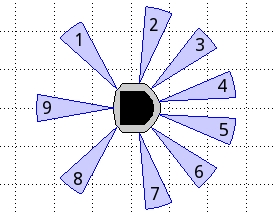
\includegraphics[bb=0 0 274 214,scale=0.6]{k3sensors.png}
 % k3sensors.png: 274x214 pixel, 72dpi, 9.66x7.55 cm, bb=0 0 274 214
 \caption{IR range sensor configuration}
 \label{fig:k3sensors}
\end{figure}




\subsection*{IR Range Sensors}
For the purpose of the homeworks and projects in the class, you will have access to the array of nine IR sensors that encompass the K3. IR range sensors are effective in the range $0.02$ m to $0.2$ m only. However, the IR sensors return raw values in the range of $[18,3960]$ instead of the measured distances. Figure \ref{fig:irvalues} demonstrates the function that maps these sensors values to distances.

\begin{figure}
 \centering
 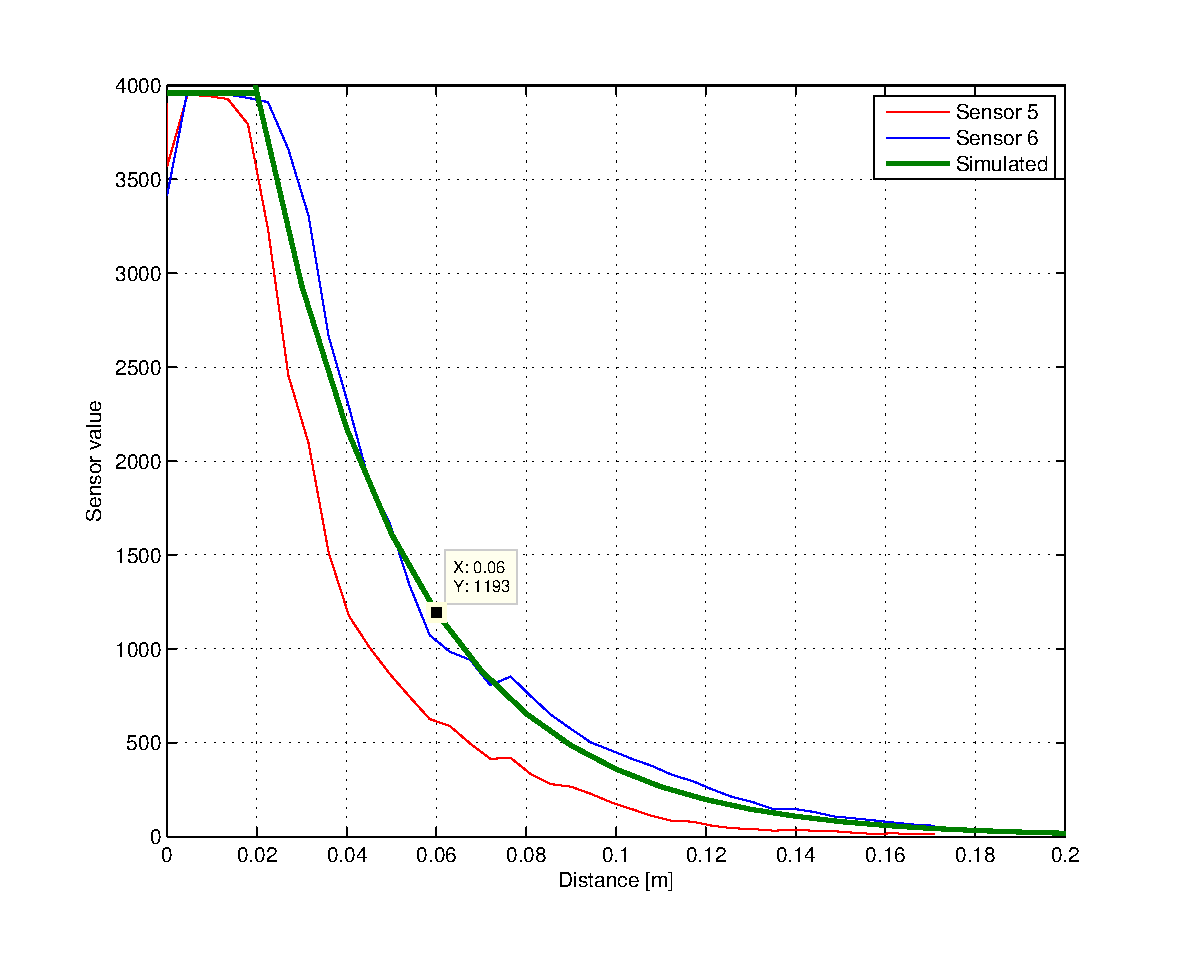
\includegraphics[scale=0.5]{./ir_actual.eps}
 % ir_actual.eps: 0x0 pixel, 300dpi, 0.00x0.00 cm, bb=   27   174   583   617
 \caption{Sensor values vs. Measured Distance}
 \label{fig:irvalues}
\end{figure}

The green plot represents the sensor model used in the simulator, while the blue and red plots show the sensor response of two different IR sensors (under different ambient lighting levels). The effect of ambient lighting (and other sources of noise) are \textbf{not} modelled in the simulator, but will be apparent on the actual hardware.

The function that maps distances, denoted by $\Delta$, to sensor values is the following piecewise function:
\begin{equation}
 f(\Delta) =
\begin{cases}
3960, & \text{if } 0\text{m} \leq \Delta \leq 0.02\text{m} \\
\lfloor3960e^{-30(\Delta-0.02)}\rfloor, & \text{if } 0.02\text{m} \leq \Delta \leq 0.2\text{m}
\end{cases}
\end{equation}

Your controller can access the IR array through the \texttt{robot} object that is passed into the \texttt{execute} function. For example,
\begin{verbatim}
 for i=1:9
    fprintf('IR #%d has a value of %d.\n', i, robot.ir_array(i).get_range());
 end
\end{verbatim}

The orientation (relative to the body of the K3, as shown in figure \ref{fig:k3sensors}) of IR sensors 1 through 9 is $128^\circ, 75^\circ, 42^\circ$, $13^\circ, -13^\circ, -42^\circ, -75^\circ, -128^\circ$, and $180^\circ$, respectively.

\subsection*{Ultrasonic Range Sensors}
The ultrasonice range sensors have a sensing range of $0.2$m to $4$m, but are not available in the simulator.

\subsection*{Differential Wheel Drive}
Since the K3 has a differential wheel drive (i.e., is not a unicyle), it has to be controlled by specifying the rotational velocities of the right and left wheel. These velocities are computed by a transformation from $(v,\omega)$ to $(v_r,v_\ell)$. Recall that the dynamics of the unicycle are defined as,
\begin{equation}
 \begin{split}
   \dot{x} &= vcos(\theta) \\
   \dot{y} &= vsin(\theta) \\
   \dot{\theta} &= \omega.
 \end{split}
\end{equation}
The dynamics of the differential drive are defined as,
\begin{equation}
 \begin{split}
  \dot{x} &= \frac{R}{2}(v_r+v_\ell)cos(\theta) \\
  \dot{y} &= \frac{R}{2}(v_r+v_\ell)sin(\theta) \\
  \dot{\theta} &= \frac{R}{L}(v_r-v_\ell),
 \end{split}
\end{equation}
where $R$ is the radius of the wheels and $L$ is the distance between the wheels.

The speed of the K3 can be set in the following way assuming that you have implemented the \texttt{uni\_to\_diff} function, which transforms $(v,\omega)$ to $(v_r,v_\ell)$:
\begin{verbatim}
 v = 0.15; % m/s
 w = pi/4; % rad/s
 % Transform from v,w to v_r,v_l and set the speed of the robot
 [vel_r, vel_l] = obj.robot.dynamics.uni_to_diff(robot,v,w);
\end{verbatim}


\subsection*{Wheel Encoders}
Each of the wheels is outfitted with a wheel encoder that increments or decrements a tick counter depending on whether the wheel is moving forward or backwards, respectively. Wheel encoders may be used to infer the relative pose of the robot. This inference is called \textbf{odometry}. The relevant information needed for odometry is the radius of the wheel, the distance between the wheels, and the number of ticks per revolution of the wheel.

\begin{verbatim}
 R = robot.wheel_radius; % radius of the wheel
 L = robot.wheel_base_length; % distance between the wheels
 tpr = robot.encoders(1).ticks_per_rev; % ticks per revolution for the right wheel

 fprintf('The right wheel has a tick count of %d\n', robot.encoders(1).state);
 fprintf('The left wheel has a tick count of %d\n', robot.encoders(2).state);
\end{verbatim}

\section*{Simulator}

Start the simulator with the \texttt{launch} command in MATLAB.

\begin{figure}
 \centering
 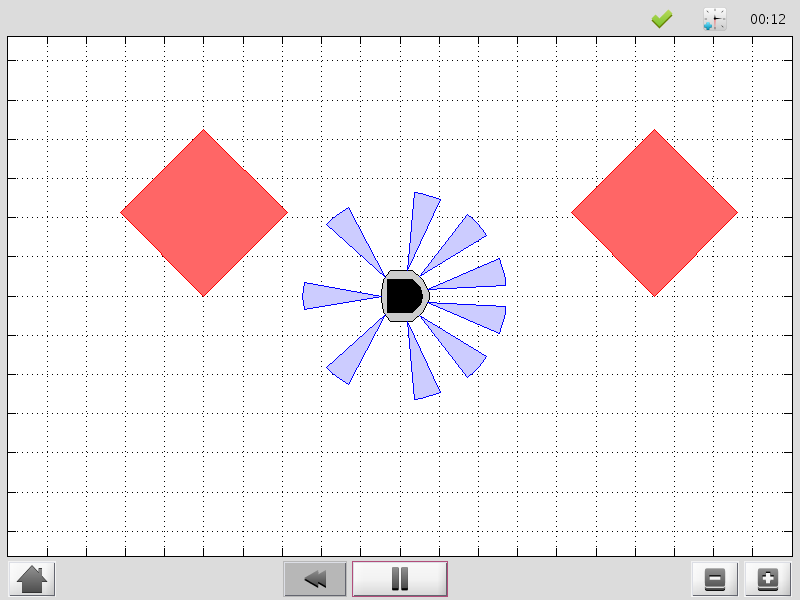
\includegraphics[scale=0.35]{simiam.png}
 \caption{Simulator}
 \label{fig:k3_sim}
\end{figure}

Figure \ref{fig:k3_sim} is a screenshot of the graphical user interface (GUI) of the simulator. The GUI can be controlled by the bottom row of buttons (or their equivalent keyboard shortcuts). The first button is the \textit{Home} button \texttt{[h]} and returns you to the home screen. The second button is the \textit{Rewind} button and resets the simulation. The third button is the \textit{Play} button \texttt{[p]}, which can be used to play and pause the simulation. The set of \textit{Zoom} buttons \texttt{[[,]]} or the mouse scroll wheel allows you to zoom in and out to get a better view of the simulation. The set of \textit{Pan} buttons \texttt{[left,right,up,down]} can be used to pan around the environment, or alternatively, Clicking, holding, and moving the mouse allows you to pan too. \textit{Track} button \texttt{[c]} can be used to toggle between a fixed camera view and a view that tracks the movement of the robot. You can also simply click on a robot to follow it.

\section*{Homeworks}

The following sections serve as a tutorial for getting through the simulator portions of the homeworks.

\subsection*{Homework 0}
The first homework asks you to implement odometry in the \texttt{+simiam/+controller/+khepera3/K3Supervisor.m} file, as well as, the transformation from $(v,\omega)$ to $(v_r,v_\ell)$ in the \texttt{+simiam/+robot/+dynamics/DifferentialDrive.m} file. Since odometry and this particular transformation will be used in all of your controllers, make sure to implement these correctly.

To test odometry and your transformation, you will likely want to edit \texttt{+simiam/+controller/GoToGoal.m} and implement a P-regulator. Similarily, for converting raw IR values to distances, edit \texttt{+simiam/+controller/}
\texttt{AvoidObstacle.m}.

\subsection*{Project 1}
The first project requires you to steer the robot to some desired angle (\texttt{theta\_d}). You will need to implement a PID regulator that achieves this quickly and smoothly. Edit \texttt{+simiam/+controller/GoToAngle.m} and implement the PID controller there. Remember, \texttt{execute} is called once every timestep \texttt{dt}, so will probably want to create variable under \texttt{properties} to save a previous error or soemthing else you want to use during the next iteration. In \texttt{+simiam/+controller/+khepera3/K3Supervisor.m}, adjust the desired angle \texttt{inputs.theta\_d = pi/4;} to make sure it works more than just the default. Also, remember to implement homework 0 before you start with this project!

\subsection*{Project 2}
The second project requires you to drive the robot to a series of given locations \texttt{x\_g} and \texttt{y\_g}. These locations are specified in \texttt{K3Supervisor.m} as a matrix, where each row corresponds to a goal and the columns correspond to the x and y location, see: \texttt{obj.goal\_list}. \texttt{obj.goal\_index} should keep track of which goal is being driven to. Use both of these variable, plus the current location of the robot to implement some simple logic that will cause the robot to drive to all three goals and then stop. \texttt{K3Supervisor.m} already has some \textbf{pseudocode} to give you an idea how this could be achieved. Feel free to implement your own logic!

The actual go-to-goal behavior needs to be implement in \texttt{GoToGoal.m}. It is recommended that you implement a PID regulator that steers the robot to the goal with a constant linear velocity. If you'd like, you may experiment with regulating the linear velocity too. The objective is for the robot to drive to all goal points and stop as close as possible to the final goal point.

\subsection*{Project 3}
The third project requires you to drive the robot away from obstacles in the environment. The robot should just drive straight when there are no obstacles, and once it detects an obstacle (in the simulator it will be a wall) it should avoid colliding with it. Compute $(v,\omega)$ that can achieve this obstacle avoiding behavior.

Hint: You may want to think about obstacle avoidance in terms of computing a vector that points away from the obstacle, and using this vector in a similar way as the go-to-goal vector to control the robot.

You may also want to think about filtering the IR measurements and/or adding a threshold for obstacle avoidance as you design this behavior.

The obstacle avoidance behavior should be implemented in \texttt{+simiam/+controller/AvoidObstacles.m}. This requires you to also properly implement the IR raw values to meters conversion in \texttt{get\_ir\_distances} in \texttt{+simiam/+robot/Khepera3.m} (refer back to homework 0 for more details).

\subsection*{Project 4}
The fourth project requires you to drive the robot to a series of goal locations without colliding with any of the obstacles in the environment. You will test two strategies:
\begin{enumerate}
  \item In \texttt{+simiam/+controller/AOandGTG.m}, implement a blend of the go-to-goal and avoid-obstacles behaviors by combining the two controllers in a meaningful way.
  \item In \texttt{+simiam/+controller/+khepera3/K3Supervisor.m}, implement switching logic that \textbf{only} switches the robot between the go-to-goal controller defined in \texttt{GoToGoal.m} and the avoid-obstacles controller defined in \texttt{AvoidObstacles.m}. Use the \texttt{switch\_controller} function to switch between two controllers.
\end{enumerate}

Think about the advantage and disadvantages of both strategies and come up with a switching logic that takes advantage of all three controllers.

\end{document}
